% Chapter 7

\chapter{Error Analysis and Quality Assurance} % Main chapter title
There are various sources of systematic error that could contribute to uncertainty in this measurement. These include certainty in how the event plane was determined (sect. \ref{secteperr}), how well the event centrality can be determined (sect. \ref{sectcenterr}), various uncertainties pertaining to the identification of the particles (sect. \ref{sectpiderr}), and the effects of detector acceptance (sect. \ref{sectaccepterr}). In this chapter I will quantify the uncertainty for each of these contributions and then use these values to find the possible variance in the flow measurement due to these uncertainties. It will be shown that event plane resolution and PID systematics due to Gaussian fitting dominate and other errors are negligible.

\section{Event Plane Resolution}
\label{secteperr}
\begin{table}[htbp!]
\centering
\caption{Event Plane Resolution for MPC, BBC, and RXNP. Resolution.}
\label{EPrestable}
\begin{tabular}{lllll}
\textbf{}                                    & \multicolumn{4}{c}{{\ul \textbf{Centrality}}}                                                                                                                              \\ \hline
\multicolumn{1}{|l|}{\textbf{Detector}} & \multicolumn{1}{c|}{\textbf{0-5\%}}      & \multicolumn{1}{c|}{\textbf{5-10\%}}      & \multicolumn{1}{c|}{\textbf{10-15\%}}    & \multicolumn{1}{c|}{\textbf{15-20\%}}    \\ \hline
\multicolumn{1}{|l|}{\textbf{BBC}}           & \multicolumn{1}{l|}{0.12821$\pm$0.00536} & \multicolumn{1}{l|}{0.19337$\pm$0.005387} & \multicolumn{1}{l|}{0.07522$\pm$0.00538} & \multicolumn{1}{l|}{0.08759$\pm$0.00538} \\ \hline
\multicolumn{1}{|l|}{\textbf{MPC}}           & \multicolumn{1}{l|}{0.25551$\pm$0.00537} & \multicolumn{1}{l|}{0.10140$\pm$0.005374} & \multicolumn{1}{l|}{0.21927$\pm$0.00537} & \multicolumn{1}{l|}{0.38086$\pm$0.00538} \\ \hline
\multicolumn{1}{|l|}{\textbf{RXN.IN}}        & \multicolumn{1}{l|}{0.14250$\pm$0.00536} & \multicolumn{1}{l|}{0.05626$\pm$0.005380} & \multicolumn{1}{l|}{0.17503$\pm$0.00538} & \multicolumn{1}{l|}{0.10996$\pm$0.00538} \\ \hline
\multicolumn{1}{|l|}{\textbf{RXN.OUT}}       & \multicolumn{1}{l|}{0.01691$\pm$0.00536} & \multicolumn{1}{l|}{0.10058$\pm$0.005389} & \multicolumn{1}{l|}{0.12035$\pm$0.00539} & \multicolumn{1}{l|}{0.02571$\pm$0.00538} \\ \hline
\multicolumn{1}{|l|}{\textbf{RXN.CMB}}       & \multicolumn{1}{l|}{0.09907$\pm$0.00535} & \multicolumn{1}{l|}{0.08638$\pm$0.005387} & \multicolumn{1}{l|}{0.12153$\pm$0.00539} & \multicolumn{1}{l|}{0.02593$\pm$0.00538} \\ \hline
\end{tabular}
\end{table}

As mentioned in section \ref{sect:epres}, the limitations of the detectors to precisely resolve the event plane result in a weaker anisotropic flow measurement which is exacerbated by the asymmetric nature of the d+Au system. By RHIC convention and PHENIX construction, the north arm is the ``deuteron-going'' side and the south side is the ``gold-going'' side, i.e. spectators from the deuteron beam hit the north arm and spectators from the gold beam hit the south arm. The significant increase in the number of nucleons in a gold nucleus result in higher track multiplicity which is used to determine the event plane. Because of this, the event plane determination using south arm detectors is significantly easier and more accurate, as evident in fig \ref{fig:evtpln}. This combination of higher track multiplicity in the south arm and a smooth flattened event plane distribution in the MPC makes it a good choice for event plane determination. Furthermore, a combinatoric calculation of the event plane resolution in the various detectors shows that the MPC has the best resolution of all the detectors possible. Additional independent measurements of the event plane are used to correct further resolution limitations in the MPC (using the Three Subevent Method, eqn. \ref{eqn3se}). The Event Plane resolution measurements displayed in table \ref{EPrestable} were determined using 5 detectors: the BBC, MPC, inner RXNP, outer RXNP, and the combined RXNP. Since any 3 detectors can be used to determine an event plane resolution correction, this correction can be calculated for the MPC using various detectors as subevent comparisons. Doing so gives a X\% variance on the MPC resolution correction.

\section{Centrality Resolution}
\label{sectcenterr}
Flow is at its strongest in most central collisions, therefore we must address the uncertainty in the centrality determination. Nagle, et al. addressed the centrality categorization in Run-8 d+Au in AN1087\citep{phenixcentrality} by correlating the charge sum in the BBC to the number of binary collisions ($\langle N_{coll} \rangle$). They found a systematic uncertainty of 7\% on the determination of $\langle N_{coll} \rangle$ for this data set for centralities from 0-20\%.

\section{Particle Identification Methods}
\label{sectpiderr}
There are three sources of error that can come from the identification of these particle species. Since the separation of signals is dependent on the time of flight and the momentum, uncertainty in either of these propagates to the error in identification. Furthermore, imperfections in the goodness of fit for the Gaussian models can systematically miscount particles contributing to further uncertainty in flow coefficients.

\subsection{Momentum Uncertainty}
Track momentum is determined by track curvature in the DC/PC1 as described in section \ref{trkrecosect}. Track curvature and certainty of this calculation is correlated to the ability to match hits in the DC and PC which is quantified by the \textit{track quality} designation. As mentioned, only tracks which have at least 3 hits in the DC and PC1 are accepted for analysis. Additionally, TOF and PC3 tracking adds additional confidence to the tracing of individual hits to reconstructed tracks. Track projections that pass the quality cut in the PC1 are projected onto the TOF and PC3 and only hits that fall within $3\sigma$ of the projected hit are accepted for analysis. Furthermore momentum reconstruction resolution has been studied with single particle simulations\citep{Mitchell:2002wu}. This resolution was shown to be linear in $p_T$ with the highest $p_T$ bin used in this analysis (5 GeV/c) having a resolution of 2\%.
 
\subsection{TOF Timing}
Since the TOF boasts a very high timing resolution and since the preamplifier gains, cable lengths, and various other systematics can affect the timing measurement from strip to strip, it is important to calibrate the response across all the strips in the TOF. Conventionally, the tracks are shifted to some expected value. Since pions are by far the most plentiful particles created in heavy ion collisions, we pick them to be our normalization. Specifically the track time distribution is plotted for each strip individually. We know the start of the event time as given by the BBC and we know the expected time of flight for a pion ($t_{\pi}$) of mass $m_{\pi}$ with a measured momentum, $p$:

\begin{equation}
t_{\pi} = \sqrt{\frac{m_{\pi}}{p^2} + \frac{1}{c^2}}.
\end{equation}

We then subtract this offset from our measured time to set the average track incidence time to around 0.

\begin{equation}
\Delta t = t_{TOF measured} - t_{collision} - t_{\pi} 
\end{equation}
 
\begin{figure}[htbp]
  \centering
    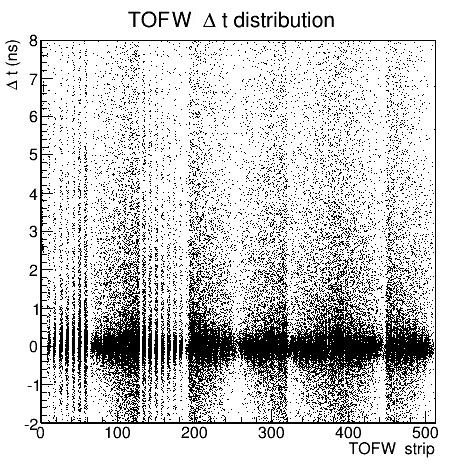
\includegraphics[width=0.5\textwidth]{evtQA/ttofwdist.JPG}
    \rule{35em}{0.5pt}
  \caption[Timing QA in the TOF.W]{Timing QA in the TOF.W, $\Delta$t vs TOF.W strip id}
  \label{fig:tofwdist}
\end{figure}

Furthermore, the TOF.W has a known resolution of $\sim 80 ps$. Propagating this error through eqn \ref{eqn:m2tof} with the known distance from the vertex of the TOF.W and a maximal value for this analysis of $p_T=5$ GeV/c, the maximum variance in $m$ due to timing capabilities is $\pm 2$ eV/c$^2$) which, when compared to the smallest mass measured ($m_{\pi}\approx$139 MeV/c$^2$), is negligible. 

\subsection{Uncertainties from Gaussian Models}
Species purity is integrated out to $2\sigma$ which accounts for 95.45\% of particles about the mean of their distribution. Therefore systematics due to mixing in the tails of the particle distributions is at most 4.55\%. Gaussian distributions do not perfectly match the particle distributions, however it can be shown that and over and under counting done by the models is uniform across each bin in $d\phi$ for a given bin of $p_T$ and only serves to shift the y-position of the flow curve a net value up or down without changing the value of the harmonic for the range $p_T \leq 3$ GeV/c. For $p_T \geq 3$ GeV/c greater systematics are evident as the widths and means of the particle distributions appear to change across different bins of $d\phi$. 

\section{Detector Acceptance}
\label{sectaccepterr}
Detectors occupy a limited and constant range in space. The ability of a detector to cover a range in space is called its \textit{acceptance}. Additionally, detectors are imperfect, there are dead channels, hot channels, edge effects, and other phenomena that can ruin the efficiency of a detector and add holes to its acceptance. Because of this, acceptance limitations of detectors can affect measurements in various analyses, however, for reasons I will discuss, a flow analysis is at best negligibly affected by detector acceptance effects. Analyses where acceptance effects are strongest are those where the coordinate system is ``static''. By this I mean that the production of analyzed tracks are studied in the lab frame coordinate system and any repeatedly missed tracks in a hole in acceptance are missed indefinitely and completely. Since event characteristics are random, by the necessity of event plane determination there is a statistical ``smearing'' that happens from the Q-vector normalization and the event plane flattening. Any holes in azimuthal coverage due to detector limitations in the lab coordinate system are smeared over by this normalization and flattening since we are performing the analysis in the event plane coordinate system which is statistically distributed and normalized. Furthermore, collaborators have studied the systematics of acceptance on $v_2$ measurements\citep{azianisystematics} by comparing $v_2$ measurements made with charged hadrons detected in TOF.E and TOF.W ($45^{\circ}$ per arm) with charged hadrons detected in full central arm acceptance ($90^{\circ}$ per arm). They found that a two-fold increase in azimuthal acceptance resulted in less than 2\% difference in flow measurements. 

\section{Summary}
Any uncertainty that would affect the value of this flow measurement would do so in one of two ways: either by shifting individual $v_2$ data points (changing inherent shape of the data set) or by changing the overall scaling of every data point in a net direction (simple scaling of entire data set). Errors that would simply shift the value of $v_2$ are the event plane resolution and centrality determination errors. Errors that would shift individual points consist of the various PID uncertainties and detector acceptance effects. The way the uncertainties in this category would shift individual data points is by changing the shape of the particle yield distribution in $d\phi$. Recall that there are two terms that parametrize the shape of the yield in $d\phi$: $yield(d\phi) = v_0 [1 + v_2 \cos 2d\phi]$. In this equation, $v_0$ corresponds to an overall shift in the function, that is to say it describes the up-and-down displacement of the whole curve and doesn't affect the general shape of it. Apart from the offset, the remaining parameter, $v_2$ describes the shape of the yield distribution in $d\phi$. Changes to the shape of this distribution that result in a change in associated $v_2$ happen when yield values are perturbed up or down in individual bins of $d\phi$. In order to study the strength of $v_2$-affecting uncertainties I will apply the variances discussed earlier in this chapter to individual points in the yield vs $d\phi$ distribution and re-fit in order to see the variances' effect on the flow coefficient. 

The particle yield is binned in six bins of $d\phi$ which therefore means that there are six points that can be perturbed systematically. Of these six points, four contribute strongly to the overall shape of the yield distribution, these are: the two end points and the two center points. In order to study the propagation of uncertainty in yield on the measured flow coefficient I created a program that can take the known values of yield in $d\phi$ and perturb them up or down by some percentage. 
\pagebreak
\pagebreak
